% Auriga theme
% https://github.com/anishathalye/auriga

\documentclass[11pt,aspectratio=169]{beamer}
\usepackage{pgfpages}
\usepackage{fancyvrb}
\usepackage{tikz}
\usepackage{pgfplots}
\usepackage{amsmath}

% Notes
%\ifnotes
%\setbeamertemplate{note page}[plain]
%\setbeameroption{show notes on second screen=right}
%\fi

\usetheme{auriga}
\usecolortheme{auriga}

% Header line
\useoutertheme[subsection=false]{miniframes}

% Footer line
\makeatletter
\def\ps@navigation@titlepage{%
  \setbeamertemplate{footline}{}
  \@nameuse{ps@navigation}
}
\addtobeamertemplate{title page}{\thispagestyle{navigation@titlepage}}{}
\pretocmd{\tableofcontents}{\thispagestyle{navigation@titlepage}}{}{}
\makeatother

% Section Slides
\AtBeginSection[]{
  \begin{frame}
  \vfill
  \centering
  \begin{beamercolorbox}[sep=8pt,center,shadow=true,rounded=true]{title}
    \usebeamerfont{title}\insertsectionhead\par%
  \end{beamercolorbox}
  \vfill
  \end{frame}
}

% adjust caption size
\newcommand\mycaption[1]{{\footnotesize #1}}

% define some colors for a consistent theme across slides
\definecolor{red}{RGB}{181, 23, 0}
\definecolor{blue}{RGB}{0, 118, 186}
\definecolor{gray}{RGB}{146, 146, 146}

% title
\title{Causal Inference \\with Heterogeneity-Robust Spatial \\Synthetic Controls}
\author{Daniel C Posmik \inst{1}}
\institute[shortinst]{\inst{1} Becker Friedman Institute for Economic Research; University of Chicago \\ E-Mail: posmikdc@uchicago.edu}


% title page
\begin{document}

{
  % rather than use the frame options [noframenumbering,plain], we make the
  % color match, so that the indicated page numbers match PDF page numbers
  \setbeamercolor{page number in head/foot}{fg=background canvas.bg}
  \begin{frame}
    \titlepage
  \end{frame}
}

% body

\begin{frame}{Table of Contents}
  \setbeamertemplate{section in toc}[sections numbered]
  \tableofcontents[hideallsubsections]
\end{frame}
\section{The Idea}
\begin{frame}{Disclaimer}
    \begin{itemize}
        \item{This is a collection of preliminary ideas.}
        \item{The purpose of this presentation is to receive constructive criticism on many of these thoughts!}
        \item{My goal is to develop this project into a paper in graduate school!}
    \end{itemize}
\end{frame}

\begin{frame}{Conventional Synthetic Controls}
  \begin{columns}
    \begin{column}{0.58\linewidth}
        \begin{itemize}
            \item{Recover causal effects when no/ few untreated comparison units are available.}
            \vspace{-7pt}
            \item{Construct synthetic control units via pre-treatment/ exogenous characteristics}
            \vspace{-7pt}
            \item{Relies on parallel trends assumption}
        \end{itemize}
    \end{column}
    \begin{column}{0.5\linewidth}
        \centering
        \includegraphics[scale = 0.3]{figures/fig.scmethod.png}\\
        \centering
        \mycaption{\cite{@abadieetal2015}: German Reunification}
    \end{column}
  \end{columns}
\end{frame}

\begin{frame}{A Three-Dimensional Extension}

\begin{itemize}
\item{\textbf{Hypothesis}: The GDP effect of German reunification is not uniform across every state}
    \begin{itemize}
        \item{Treatment effect heterogeneity?}
        \vspace{-5pt}
        \item{Complex spatial relationships?}
        \vspace{-5pt}
        \item{Information loss during data aggregation?}
    \end{itemize}
\end{itemize}

\hfill

\begin{itemize}
    \item{Spatial Synthetic Controls (SSC) adds a spatial dimension to the \textit{conventional} Synthetic Controls (SC) method}
    \begin{itemize}
        \item{Disaggregation of information in the spatial dimension}
        \vspace{-5pt}
        \item{Refine the average (ATE) to conditional (CATE) treatment effects}
        \vspace{-5pt}
        \item{Causal inference in high-dimensional space}
    \end{itemize}
\end{itemize}
\end{frame}

\begin{frame}{A Three-Dimensional Extension: Visualization}

Treatment occurs at $t_{i=0}$. Let us consider three scenarios:
\vspace{5pt}

  \begin{columns}
    % Split 1
    \begin{column}{0.33\linewidth}
      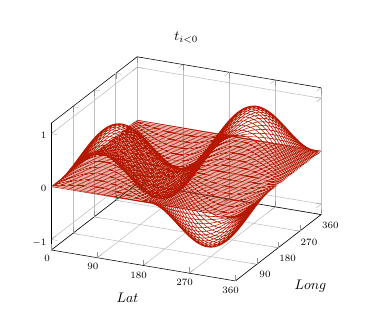
\begin{tikzpicture}[scale=0.50]
      \begin{axis} [
        title = {$t_{i<0}$},
        xtick = {0,90,...,360},
        ytick = {90,180,...,360},
        xlabel = $Lat$, ylabel = $Long$,
        ticklabel style = {font = \scriptsize},
	grid]
        \addplot3 [red, domain=0:360, samples=60] 
        	{ sin(x)*sin(y) };
        \end{axis}
        \end{tikzpicture}
        \centering{\footnotesize{Pre-treatment, no treatment response}}
    \end{column}
    % Split 2
    \begin{column}{0.33\linewidth}
      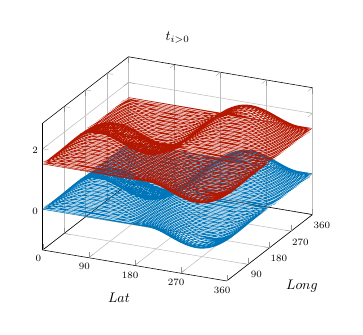
\begin{tikzpicture}[scale=0.50]
      \begin{axis} [
        title = {$t_{i>0}$},
        xtick = {0,90,...,360},
        ytick = {90,180,...,360},
        xlabel = $Lat$, ylabel = $Long$,
        ticklabel style = {font = \scriptsize},
	grid]
        \addplot3 [blue, domain=0:360, samples=60] 
        	{ sin(x)*sin(y) };
        \addplot3 [red, domain=0:360, samples=60] 
        	{ sin(x)*sin(y) + 1.5 };
        \end{axis}
        \end{tikzpicture}
        \centering{\footnotesize{Post-treatment, homogeneous response}}
    \end{column}
    % Split 3
    \begin{column}{0.33\linewidth}
      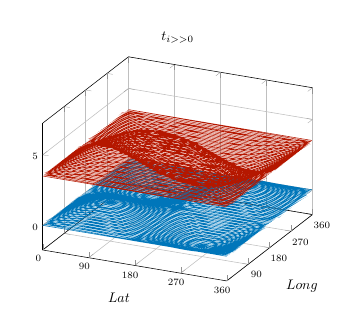
\begin{tikzpicture}[scale=0.50]
      \begin{axis} [
        title = {$t_{i>>0}$},
        xtick = {0,90,...,360},
        ytick = {90,180,...,360},
        xlabel = $Lat$, ylabel = $Long$,
        ticklabel style = {font = \scriptsize},
	grid]
        \addplot3 [blue, domain=0:360, samples=60] 
        	{ sin(x)*sin(y) };
        \addplot3 [red, domain=0:360, samples=60] 
        	{ sin(0.5*x)*3*sin(y) + 3.5 };
        \end{axis}
        \end{tikzpicture}
        \centering{\footnotesize{Post-treatment, heterogeneous response}}
    \end{column}
  \end{columns}

\end{frame}
\section{Counterfactual Prediction}

\begin{frame}{Finding a Prediction Algorithm}
    \begin{columns}
    \begin{column}{0.6\linewidth}
    Need to find a prediction algorithm to generate synthetic (counterfactual) control data post-treatment. \\
    This algorithm must be:
      \begin{enumerate}
         \item {Excellent at modeling non-linear relationships}
         \item {Robust to unobserved heterogeneity across space and time}
         \item {Suitable for high-dimensional space}
      \end{enumerate}
      \vspace{5pt}
    \footnotesize{Note: Both discrete and continuous estimands are considered. The Application section elaborates.}
    \end{column}
    \begin{column}{0.4\linewidth}
      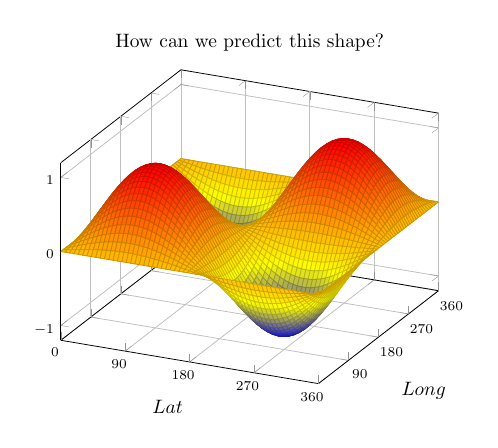
\begin{tikzpicture}[scale=0.70]
      \begin{axis} [
        title = {How can we predict this shape?},
        xtick = {0,90,...,360},
        ytick = {90,180,...,360},
        xlabel = $Lat$, ylabel = $Long$,
        ticklabel style = {font = \scriptsize},
	grid]
        \addplot3 [surf, domain=0:360, samples=60] 
        	{ sin(x)*sin(y) };
        \end{axis}
        \end{tikzpicture}
    \end{column}
  \end{columns}
\end{frame}

\begin{frame}{A Geometric Learning Approach: Graph Neural Networks}

    \begin{columns}
    \begin{column}{0.4\linewidth}
    \vspace{5pt}
      \begin{enumerate}
         \item {Invariance to Permutation, Size, and Shape: Capable of handling complex data via graph representation}
         \item {Reliable performance in non-Euclidian space: Important in high-dimensional setting}
         \item {Features and similarity: Conveys both edge and node information}
      \end{enumerate}
    \end{column}
    \begin{column}{0.6\linewidth}
      \centering
      \includegraphics[scale=0.1]{figures/gnn_summ.png}
      \caption{\footnotesize{Summary of 2-D and 3-D Graph Neural Networks}}
    \end{column}
  \end{columns}
\end{frame}

\begin{frame}{Visualizing the End Goal}

Consider treatment $Z_{it}$ occuring at $t = t^{*}$ for all locations $i$. Hypothetically, a Graph Neural Network (GNN) can predict \textcolor{cyan}{counterfactual untreated outcomes} at various locations over time:
\vspace{7pt}

  \begin{columns}
    % Split 1
    \begin{column}{0.33\linewidth}
      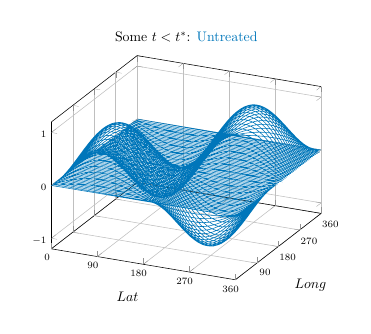
\begin{tikzpicture}[scale=0.50]
      \begin{axis} [
        title = {Some $t < t^{*}$: \textcolor{blue}{Untreated}},
        xtick = {0,90,...,360},
        ytick = {90,180,...,360},
        xlabel = $Lat$, ylabel = $Long$,
        ticklabel style = {font = \scriptsize},
	grid]
        \addplot3 [blue, domain=0:360, samples=60] 
        	{ sin(x)*sin(y) };
        \end{axis}
        \end{tikzpicture}
        \centering{\footnotesize{Pre-treatment, no treatment response, $Y_{it}(0)$}}
    \end{column}
    % Split 2
    \begin{column}{0.33\linewidth}
      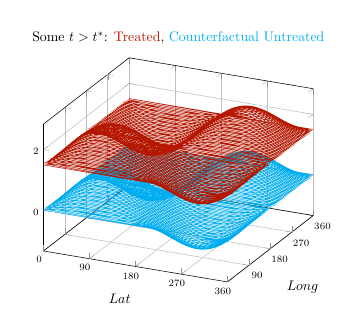
\begin{tikzpicture}[scale=0.50]
      \begin{axis} [
        title = {Some $t > t^{*}$: \textcolor{red}{Treated}, \textcolor{cyan}{Counterfactual Untreated}},
        xtick = {0,90,...,360},
        ytick = {90,180,...,360},
        xlabel = $Lat$, ylabel = $Long$,
        ticklabel style = {font = \scriptsize},
	grid]
        \addplot3 [cyan, domain=0:360, samples=60] 
        	{ sin(x)*sin(y) };
        \addplot3 [red, domain=0:360, samples=60] 
        	{ sin(x)*sin(y) + 1.5 };
        \end{axis}
        \end{tikzpicture}
        \centering{\footnotesize{Post-treatment, homogeneous response, $Y_{it}(1)$}}
    \end{column}
    % Split 3
    \begin{column}{0.33\linewidth}
      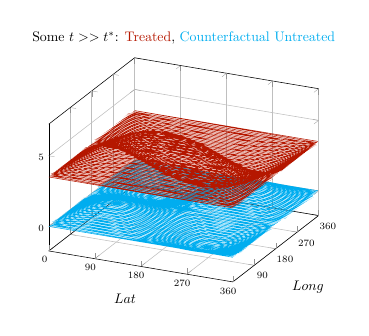
\begin{tikzpicture}[scale=0.50]
      \begin{axis} [
        title = {Some $t >> t^{*}$: \textcolor{red}{Treated}, \textcolor{cyan}{Counterfactual Untreated}},
        xtick = {0,90,...,360},
        ytick = {90,180,...,360},
        xlabel = $Lat$, ylabel = $Long$,
        ticklabel style = {font = \scriptsize},
	grid]
        \addplot3 [cyan, domain=0:360, samples=60] 
        	{ sin(x)*sin(y) };
        \addplot3 [red, domain=0:360, samples=60] 
        	{ sin(0.5*x)*3*sin(y) + 3.5 };
        \end{axis}
        \end{tikzpicture}
        \centering{\footnotesize{Post-treatment, heterogeneous response, $Y_{it}(1)$}}
    \end{column}
  \end{columns}
\end{frame}
\section{Choosing Comparison Units}

\begin{frame}{Motivation}
Let us decompose the treatment effect $\tau$. \\
\vspace{5pt}
\begin{itemize}
    \item $Y_{it}^{(1)}$: The set of treated outcomes is observed. Assuming the absence of measurement error, the data are accurate. 
    \vspace{-7pt}
    \item $Y_{it}^{(0)}$: The set of untreated potential outcomes are not observed. Bias and inaccuracies likely stem from (i) prediction errors of the untreated data but also (ii) the choice of untreated units we choose to compare our observed treated unit with.
\end{itemize}

Therefore, even if we have generated reliable synthetic data for the untreated outcomes, that leaves us with one important choice:\\ 
\vspace{5pt}
\centering
\textbf{Which control units $Y_{it}^{(0)}$ do we compare our treated unit $Y_{it}^{(1)}$ with to obtain $\tau$?}
\end{frame}

\begin{frame}{Context}
Intuitively, this problem equates to not wanting to compare apples to oranges. \\
\vspace{5pt}
\begin{enumerate}
    \item Using a set of covariates $X_{it}$ to control for confounders (Pollmann WP)
        \begin{itemize}
            \item Pros: It is easy to overlay spatial distributions of covariates in a map (Think: Each covariate is a separate heatmap)
            \item Cons: Curse of dimensionality; does not capture unobserved heterogeneity
        \end{itemize}
    \item Using the k nearest units as comparison units
        \begin{itemize}
            \item Pros: It is easy to implement and intuitive
            \item Cons: Disregards more complex spatial relationships; breaks in higher dimensions; inherently arbitrary
        \end{itemize}
    \item Using spatial first differences (Druckenmiller \& Hsiang, 2019)
        \begin{itemize}
            \item Pros: It does account for unobserved heterogeneity (Think: Mini RDs between spatially adjacent units); No functional form assumptions and purely data-driven
            \item Cons: Breaks in higher dimensions
        \end{itemize}
\end{enumerate}
\end{frame}

\begin{frame}{The Spatial First Differences Idea}

Spatial first differences do remove unobserved heterogeneity, great!\\
\vspace{5pt}
\centering
\includegraphics[scale=0.67]{figures/spatialfd.png}
\caption{\footnotesize{Druckenmiller \& Hsiang, 2018}}\\
\vspace{7pt}
\Rightarrow \textbf{ However, this approach breaks down when we want to account for a (non-pooled) time dimension. Can we borrow any ML tools to deal with this high-dimensional problem?}
\end{frame}

\begin{frame}{A Geometric Learning Approach}

\begin{columns}
% Split 1
\begin{column}{0.45\linewidth}
\begin{itemize}
    \item Let us consider a graph where the nodes correspond to the units, and the edges between them represent the spatial differences. 
    \vspace{-7pt}
    \item Then, the length of the edges can be a measure of the similarity of units under identical treatment status. 
    \vspace{-7pt}
    \item When adding the time dimension, the graph consists of both spatial and temporal edges.
\end{itemize}
\end{column}
% Split 2
\begin{column}{0.6\linewidth}
\centering
\includegraphics[scale=0.33]{figures/gnn.png}
\caption{\footnotesize{Kapoor, Ben et al., 2020: COVID-19 Infections}}
\end{column}
\end{columns}
\end{frame}

\begin{frame}{A Geometric Learning Approach (ctd.)}

As long as we do not compare units across treatment status, we will obtain a three-dimensional graph. The edges represent a measure of similarity - a spatial or temporal first difference, respectively that is standardized across dimensions.\\
\vspace{3pt}
\begin{columns}
    \begin{column}{0.85\linewidth}
    Formally, we can use a graph clustering algorithm to divide this 3-D graph into subsets. These k subsets will:
    \begin{itemize}
        \item Be between 1 < k < n, where 1 would include all units and n will construct a separate cluster for each unit in space and time
        \vspace{-7pt}
        \item Minimize the within-cluster average edge length: $\bar{E} = \frac{1}{k}\sum_{it}^{IT}(E)$; $\forall i \in I, t \in T.$
        \item Note: The spatial dimension shall be finely gridded. Coarse grids may omit valuable information. 
    \end{itemize}
    \end{column}
    % Split 2
    \begin{column}{0.17\linewidth}
        \includegraphics[scale=0.21]{figures/gnn_cluster.png}
        \caption{}
    \end{column}
\end{columns}
\end{frame}

\begin{frame}{Outcome and Practical Challenges}

The desired outcome is a set of k clusters within which all units are comparable across space and time. Metaphorically, we are sorting a basket of apples and oranges into two separate baskets containing apples and oranges, respectively. 

Notably, there are considerable implementation challenges:\\
\begin{itemize}
    \item As $k \rightarrow n$, $\bar{E}$ may monotonically decrease s.t. there is no $k$ that minimizes $\bar{E}$ other than $k=n$
    \vspace{-7pt}
    \item Approaches to finding this optimal k have included the elbow and silhouette methods
    \vspace{-7pt}
    \item Optimization literature may give insight into appropriate constraints, e.g., continuity, non-separability, and overlap of clusters. 
\end{itemize}
\end{frame}

\section{DiD Framework}


\begin{frame}{Group-Time Average Treatment Effects}

The \textbf{group-time average treatment effect}, $ATT(g,t)$, is a causal parameter in the context of DiD with multiple periods and multiple groups. The $ATT(g,t)$ has been approximated with the following estimators ($\tau$): \\
\vspace{5pt}
\begin{itemize}
    \item Outcome-regressions (Rubin, 1979) \\
    \vspace{3pt}
    $\tau^{reg} = N^{-1} \sum_{i=1}^{N}\{\hat{\mu_{1}}(X_{i}) - \hat{\mu_{0}}(X_{i}) \}$
    \vspace{-7pt}
    \item Inverse Probability Weighting (Rosenbaum, 1987) \\
    \vspace{3pt}
    $\tau^{ipw} = \frac{\sum_{i=1}^{N} Z_i Y_i / \hat{e}(X_i)}{\sum_{i=1}^{N} Z_i / \hat{e}(X_i)} - \frac{\sum_{i=1}^{N} (1-Z_i) Y_i / \{1 - \hat{e}(X_i)\}}{\sum_{i=1}^{N} (1-Z_i) / \{1 - \hat{e}(X_i)\}}$ \\
    \vspace{3pt}
    \footnotesize{where $\hat{e}$ is the estimated propensity score.} 
    \vspace{-7pt}
    \item Doubly-Robust Methods \\
    \vspace{3pt}
    $\tau^{dr} = \tau^{reg} + N^{-1} \sum_{i=1}^{N} \{ \frac{Z_i R_i}{\hat{e}(X_i)} - \frac{(1-Z_i) R_i}{1 - \hat{e}(X_i)} \}$ \\
    \vspace{3pt}
    \footnotesize{where $R_i = Y_i - \mu_{Z_{i}}(X_i)$ denotes the residual from outcome modeling.}
\end{itemize}
\end{frame}

\begin{frame}{A new estimator}
... blah blah blah ...
\end{frame}

\begin{frame}{Defining the g in ATT(g,t)}
Frequently, units are clustered before inference. For example, the ATT(g,t) may be evaluated on the zip code level. However, this can bias the estimation of a treatment effect because:
\vspace{5pt}

\begin{enumerate}
    \item Pre-defined borders may not be applicable in treatment context
    \item Biases of policymakers may be imposed on the study ex ante
\end{enumerate}
\vspace{5pt}

We can overcome this issue by \textbf{inferring the clusters ex post}, i.e. after obtaining individual-level treatment effects. Formally, we ...
\vspace{5pt}

\begin{enumerate}
    \item Measure idiosyncratic treatment effects over space and time, acknowledging that there will be missing treatment effects. 
    \item Interpolate missing treatment effects using the discrete subset we did measure.
    \item Divide the continuous set of treatment effects into k distinct clusters which represent approximations of the ATT(g,t) that are robust to spatial heterogeneity.  
\end{enumerate} 
\end{frame}

\begin{frame}{Defining the g in ATT(g,t): A Visualization}
The existence of zip codes can be attributed to a variety of historical, political, and administrative factors, but these divisions do not necessarily correspond to a population that is homogeneous in their treatment response.
\vspace{5pt}

  \begin{columns}
    % Split 1
    \begin{column}{0.4\linewidth}
    \centering
      \includegraphics[scale=0.16]{figures/sf_zipcodes_exante.jpeg}
      \caption{\footnotesize{Ex Ante Comparison: Apples to Oranges}}
    \end{column}
    % Split 2
    \begin{column}{0.1\linewidth}
    \centering
      \Rightarrow
    \end{column}
    % Split 3
    \begin{column}{0.4\linewidth}
    \centering
      \includegraphics[scale=0.16]{figures/sf_zipcodes_expost.jpeg}
      \caption{\footnotesize{Ex Post Comparison: Apples to Apples}}
    \end{column}
  \end{columns}
\end{frame}

\begin{frame}{Control Strategy}
    Overlaying distributions of controls. This should also inform the clusters.
    More specifically: What if I can build the clusters based on all the covariates I consider and then represent them in a lower dimension in space???
\end{frame}

\begin{frame}{Limitations}
\begin{itemize}
    \item Vulnerable to structural differences in treatment effect density. Assumes the measurement of treatment effects across space and time distributed at random. 
\end{itemize}
    
\end{frame}
\section{Heatwave Application}

\begin{frame}{Motivation}

  \begin{columns}
    \begin{column}{0.6\linewidth}
      \begin{itemize}
        \item Measuring the effect of climate disasters
            \begin{itemize}
            \item Experimental approaches - if not unethical - are nearly impossible
            \item Researchers are stuck with observational data
            \item Recovering robust causal effects is critical policy input
            \end{itemize}
      \end{itemize}
    \end{column}
    \begin{column}{0.4\linewidth}
      \includegraphics[scale=0.1]{figures/california-heatwave-2020-nasa-eo.jpeg}
      \caption{}
    \end{column}
  \end{columns}

\vspace{7pt}
\begin{center}
    Application: How do we measure the effect of heat waves on community health?
\end{center}

  \note{
    This slide has notes too.
  }

\end{frame}

\begin{frame}{Colorado Cell Phone Ping Data}
- E&E Lab cell phone ping data
- Data Use: Assign unit treated if it moved to hospital
\end{frame}

% Appendix----------------------------------------------------------------
\appendix

% References--------------------------------------------------------------
\begin{frame}[allowframebreaks]{References}
  \bibliography{main.bib}
  \bibliographystyle{apalike}
\end{frame}

\end{document}
